\section{Domain Name System Service}
\label{sec:dns}

\subsection{Design}

Domain Name System (DNS)\citep{rfc1035} translates IP addresses to domain names and vice versa.
In contrast to hard-to-remember IP addresses, short and meaningful domain names (eg. \texttt{lboro.ac.uk} for Loughborough University in UK) are more convient for Internet users. 
Additionally, the service providers can change the IP addresses of servers without re-notifying their customers.

In BT Network, there are two DNS servers, one primary master server and the other secondary. Primary master server is deployed at Laptop 3 (BT003) and secondary master server is at Laptop 1 (BT001). 
The rationale is that when the primary becomes unavailable, the secondary can be the backup domain name server.

Both are authoritative of domain \texttt{bt.lboro}. \textbf{Each laptop in the network has a corresponding domain name. For example, the domain name of Laptop 1 (BT001) is \texttt{bt001.bt.lboro}. In addition, both \texttt{A} and \texttt{AAAA} records of \texttt{bt.lboro} point to Laptop 1 while the MX record points to Laptop 3.}

The two DNS servers are also connected to the central DNS server, which is authoritative of domain \texttt{lboro}.



\subsection{Implementation}

Install \texttt{bind9} package and \texttt{dnsutils} package on Laptop 1 (BT001) and Laptop 3 (BT001) using the following commands. All DNS configurations are all stored in folder \texttt{/etc/bind}.

\begin{lstlisting}
sudo apt-get install bind9
sudo apt-get install dnsutils
\end{lstlisting}


On the primary DNS server, forward unknown DNS requests to central DNS server by adding this line to file \texttt{named.conf.options}.

\begin{lstlisting}
forwarders { 10.2.2.1; };
\end{lstlisting}



The following lines are added to file \texttt{/etc/bind/named.conf.local}.

The zone section defines the type of the DNS server and it is stored in a file mentioned in the 'file' field. 
The 'allow-transfer' field defines a match list which has IP addresses that are allowed to do transfer and copy operations to the zone information with the server. 
The 'allow-notify' field defines an IP addresses match list that is allowed to notify this server and implicitly update the zone.
In this case, both fields should be the IP address of the secondary DNS server (Laptop 1).

The first zone is a forward zone which translate the domain name to IP address. The zone name of it is the selected domain name \texttt{bt.lboro}. 
The second zone is the reverse zone which translate the IP address to domain name. The zone name of it should be the fixed IP prefix part and host part. In this case, the name is \texttt{23.in-addr.arpa}.


\begin{lstlisting}
zone “bt.lboro’ {
	type master;
	file “/etc/bind/db.bt.lboro”;
	allow-transfer { 23.0.0.2; };
	also-notify { 23.0.0.2; };
};

zone “23.in-addr.arpa’ {
	type master;
	file “/etc/bind/db.23”;
	allow-transfer { 23.0.0.2; };
	also-notify { 23.0.0.2; };
};
\end{lstlisting}

Then, the files related to forward zone and reverse zone are edited. 

The contents of file \texttt{db.bt.lboro} which is shown in Figure \ref{fig:db-bt-lboro} defines the forward DNS configuration.

\begin{figure*}[ht!]
% TODO
\caption{Contents of Forward DNS Configuration File Named \texttt{db.bt.lboro}}
\lable{fig:db-bt-lboro}
\end{figure*}


Serial number is the version number of this file and it should be increased after changing the file. 
For each line of records, the prefix (eg. \texttt{bt001}), domain type (eg. \texttt{A}) and value (eg. \texttt{23.0.0.2}) are specified.


\begin{figure*}[ht!]
% TODO
\caption{Contents of Reverse DNS Configuration File Named \texttt{db.23}}
\lable{fig:db-23}
\end{figure*}

Figure \ref{fig:db-23} shows the configuration for the reverse zone. 
The serial number needs to be increased on each change as well. 
For each line of records, the first column of match list should be reverse host part of IP address. 
For example, the IP address of Laptop 1 (BT001) is \texttt{23.0.0.2} and the host part of it is \texttt{0.0.2}. Therefore, the reverse host part of it should be \texttt{2.0.0}. 

For each A record in forward configurations, a PTR records should be added to the reverse configuration.

When all configurations for DNS server are completed, use following commands to restart \texttt{bind9} service to take effect.

\begin{lstlisting}
service bind9 restart
\end{lstlisting}

As for secondary master, Laptop 1 (BT001) only needs to add the following lines to the file \texttt{/etc/bind/named.conf.local}, which specify both forward and reverse DNS zones and Laptop 3 as their master server.

\begin{lstlisting}
zone “bt.lboro’ {
			type slave;
			file “db.bt.lboro”;
			masters { 23.0.0.34; };
};

zone “23.in-addr.arpa’ {
			type slave;
			file “db.23”;
			masters { 23.0.0.34; }
};
\end{lstlisting}

Restart \texttt{bind9} service for configurations to take effect.

\begin{lstlisting}
service bind9 restart
\end{lstlisting}

Now, Laptop 2 should be able to receive DNS records from the master server and act as a secondary DNS server.




\subsection{Evaluation}

The command \texttt{dig} is used to query DNS records on Laptop 2 for evaluation. In Figure \ref{fig:dns-dig}, DNS records of \texttt{bt.lboro} and \texttt{www.bt.lboro} are "digged" and correct answers are returned by DNS servers.

\begin{figure*}[ht!]
    \centering
    \begin{subfigure}[b]{0.67\textwidth}
        \centering
        \includegraphics[width=\linewidth]{dns-dig-1}
        \caption{\texttt{bt.lboro}}
    \end{subfigure}
    \hfill
    \begin{minipage}[b]{0.3\textwidth}
	    \begin{subfigure}[b]{\linewidth}
	        \centering
	        \includegraphics[width=\linewidth]{dns-dig-2}
	        \caption{\texttt{www.bt.lboro}}
	    \end{subfigure}
	    \\
	    \begin{subfigure}[b]{\linewidth}
	        \centering
	        \includegraphics[width=\linewidth]{dns-dig-3}
	        \caption{\texttt{MX} Records of \texttt{bt.lboro}}
	    \end{subfigure}
	\end{minipage}
    \caption{Querying DNS Records for \texttt{bt.lboro} and \texttt{www.bt.lboro} on Laptop 2.}
    \label{fig:dns-dig}
\end{figure*}

In addition, DNS records of \texttt{bt001.bt.lboro}, \texttt{bt002.bt.lboro} and \texttt{bt003.bt.lboro} are "digged" on Laptop 2 as well. In Figure \ref{fig:dns-dig-laptops}, correct answers are returned by DNS servers.


\begin{figure*}[ht!]
    \centering
    \begin{subfigure}[b]{0.67\textwidth}
        \centering
        \includegraphics[width=\linewidth]{dns-dig-laptops-1}
        \caption{\texttt{bt001.bt.lboro}}
    \end{subfigure}
    \hfill
    \begin{minipage}[b]{0.3\textwidth}
	    \begin{subfigure}[b]{\linewidth}
	        \centering
	        \includegraphics[width=\linewidth]{dns-dig-laptops-2}
	        \caption{\texttt{bt002.bt.lboro}}
	    \end{subfigure}
	    \\
	    \begin{subfigure}[b]{\linewidth}
	        \centering
	        \includegraphics[width=\linewidth]{dns-dig-laptops-3}
	        \caption{\texttt{bt003.bt.lboro}}
	    \end{subfigure}
	\end{minipage}
    \caption{Querying DNS Records for sub-domains of \texttt{bt.lboro} on Laptop 2.}
    \label{fig:dns-dig-laptops}
\end{figure*}



In terms of IPv6 addresses, DNS \texttt{AAAA} records of \texttt{bt001.bt.lboro}, \texttt{bt002.bt.lboro} and \texttt{bt003.bt.lboro} are "digged" on Laptop 2 as well. In Figure \ref{fig:dns-dig-aaaa}, correct answers are returned by DNS servers.

\begin{figure*}[ht!]
    \centering
    \begin{subfigure}[b]{0.67\textwidth}
        \centering
        \includegraphics[width=\linewidth]{dns-dig-aaaa-1}
        \caption{\texttt{bt001.bt.lboro}}
    \end{subfigure}
    \hfill
    \begin{minipage}[b]{0.3\textwidth}
	    \begin{subfigure}[b]{\linewidth}
	        \centering
	        \includegraphics[width=\linewidth]{dns-dig-aaaa-2}
	        \caption{\texttt{bt002.bt.lboro}}
	    \end{subfigure}
	    \\
	    \begin{subfigure}[b]{\linewidth}
	        \centering
	        \includegraphics[width=\linewidth]{dns-dig-aaaa-3}
	        \caption{\texttt{bt003.bt.lboro}}
	    \end{subfigure}
	\end{minipage}
    \caption{Querying DNS \texttt{AAAA} Records for sub-domains of \texttt{bt.lboro} on Laptop 2.}
    \label{fig:dns-dig-aaaa}
\end{figure*}


For reverse DNS, records of Laptop 1 (\texttt{23.0.0.2}), Laptop 2 (\texttt{23.0.0.18}) and Laptop 3 (\texttt{23.0.0.34}) are "digged" on Laptop 2 as well. In Figure \ref{fig:dns-dig-reverse}, correct answers are returned by DNS servers.


\begin{figure*}[ht!]
    \centering
    \begin{subfigure}[b]{0.67\textwidth}
        \centering
        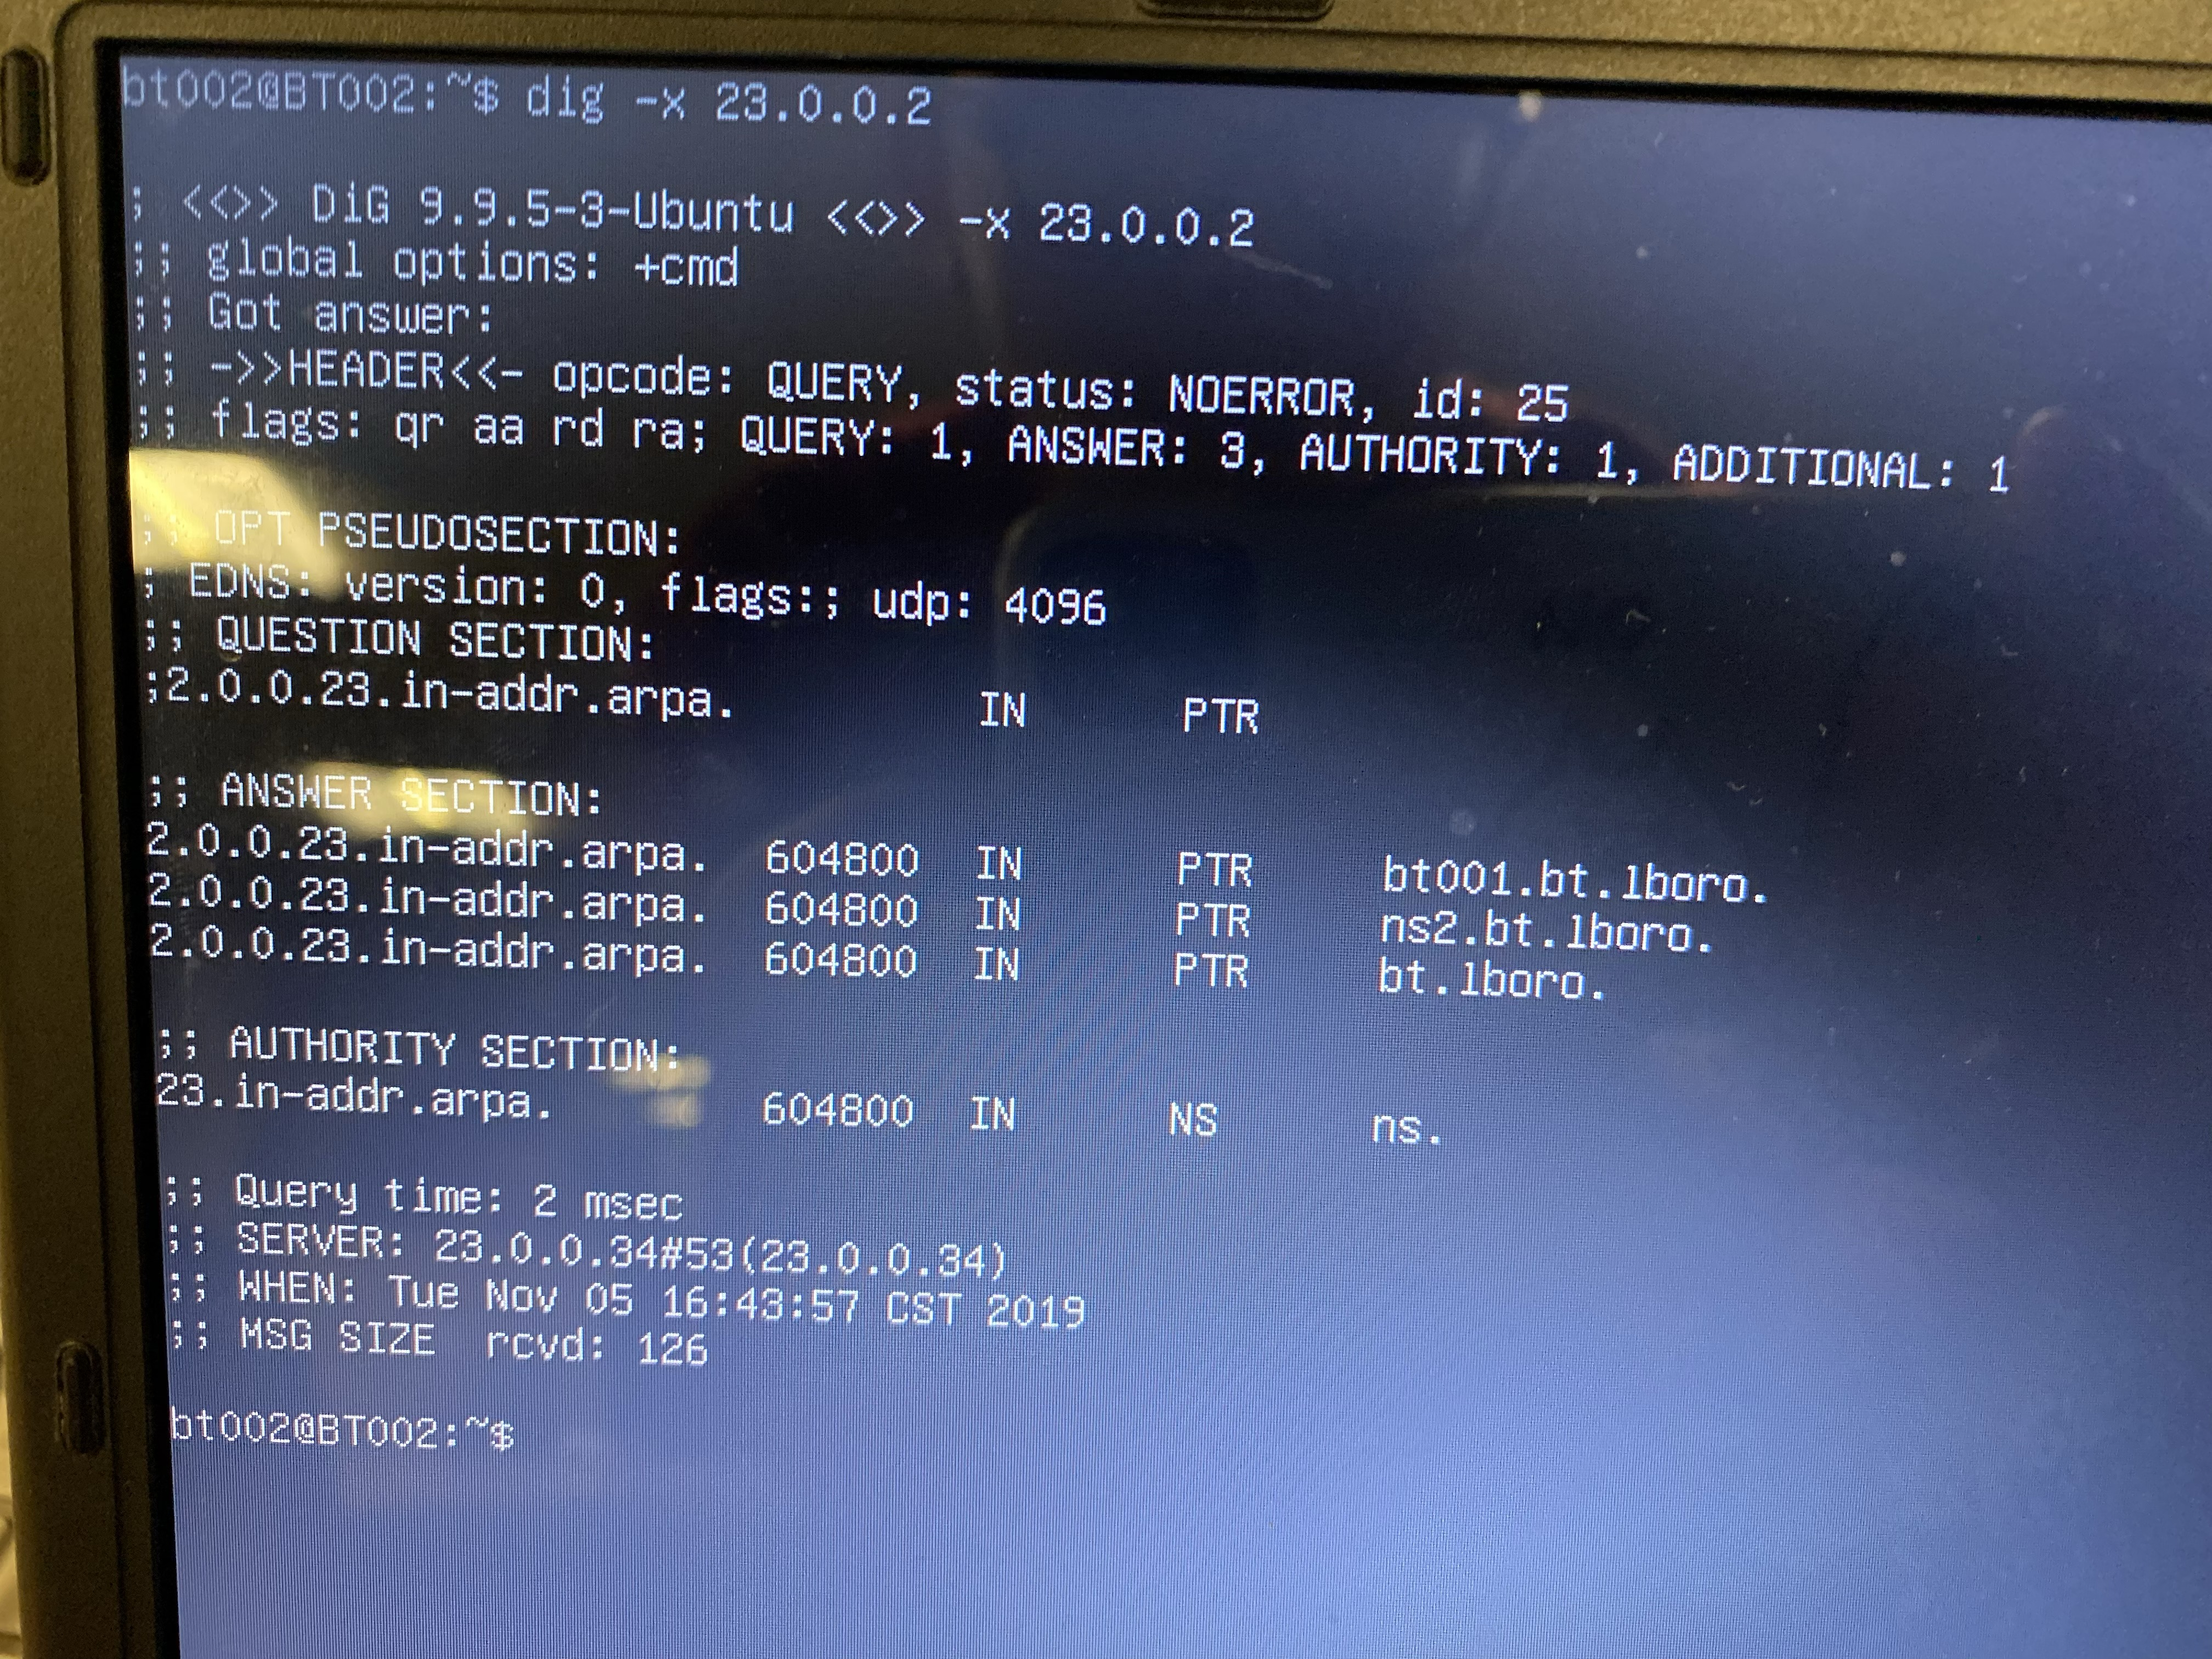
\includegraphics[width=\linewidth]{dns-dig-reverse-1}
        \caption{\texttt{23.0.0.2}}
    \end{subfigure}
    \hfill
    \begin{minipage}[b]{0.3\textwidth}
	    \begin{subfigure}[b]{\linewidth}
	        \centering
	        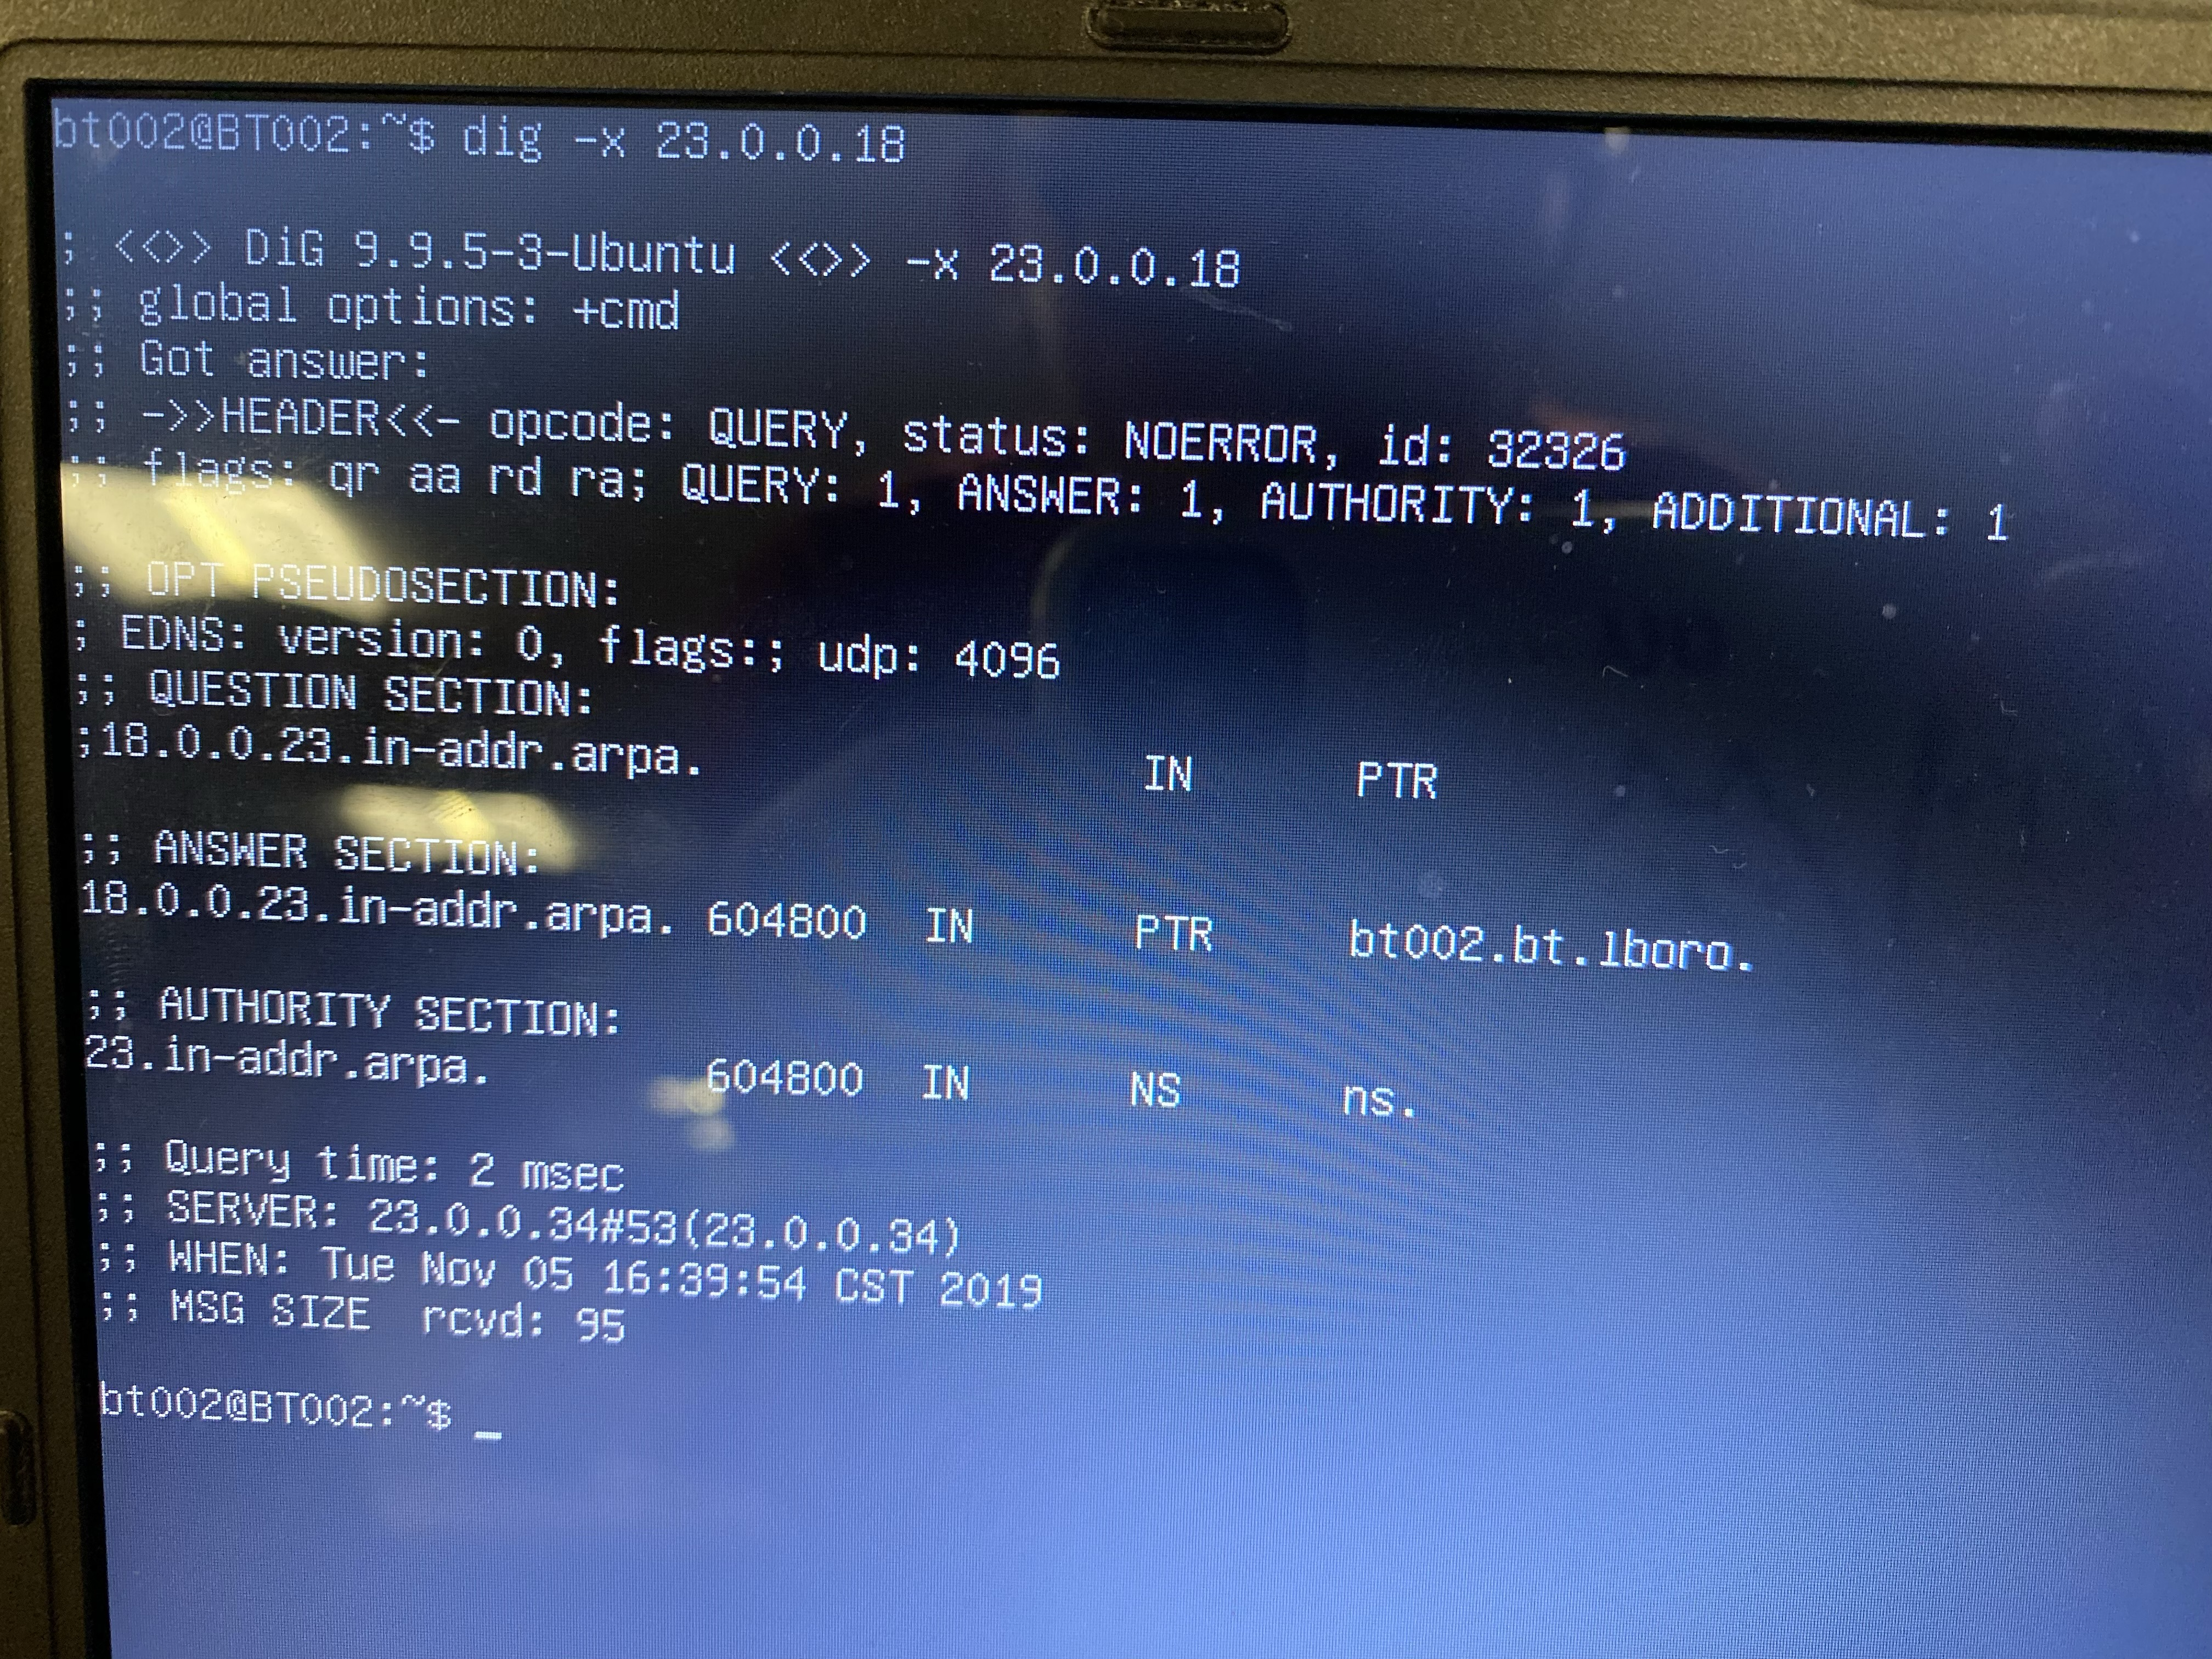
\includegraphics[width=\linewidth]{dns-dig-reverse-2}
	        \caption{\texttt{23.0.0.18}}
	    \end{subfigure}
	    \\
	    \begin{subfigure}[b]{\linewidth}
	        \centering
	        \includegraphics[width=\linewidth]{dns-dig-reverse-3}
	        \caption{\texttt{23.0.0.34}}
	    \end{subfigure}
	\end{minipage}
    \caption{Querying Reverse DNS Records for All $3$ Laptops on Laptop 2.}
    \label{fig:dns-dig-reverse}
\end{figure*}


In terms of connectivity, all three laptops are able to directly \texttt{ping} the domain name \texttt{bt.lboro}, whose DNS \texttt{A} record points to Laptop 1 (BT001, IPv4 Address: \texttt{23.0.0.2}), as shown in Figure \ref{fig:dns-ping}.

\begin{figure*}[ht!]
    \centering
    \begin{subfigure}[b]{0.67\textwidth}
        \centering
        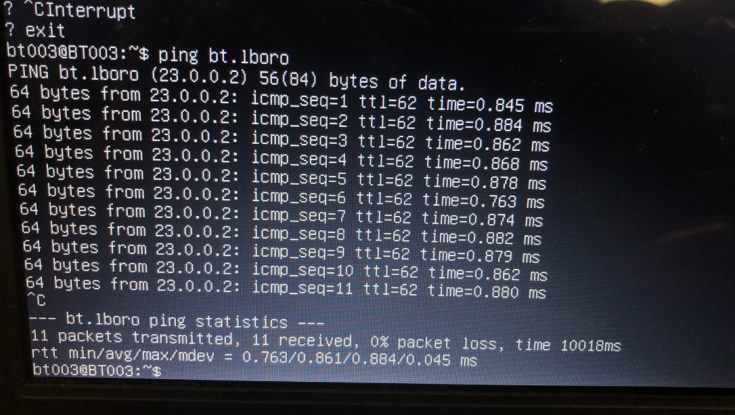
\includegraphics[width=\linewidth]{dns-ping-1}
        \caption{Laptop 1 (BT001)}
    \end{subfigure}
    \hfill
    \begin{minipage}[b]{0.3\textwidth}
	    \begin{subfigure}[b]{\linewidth}
	        \centering
	        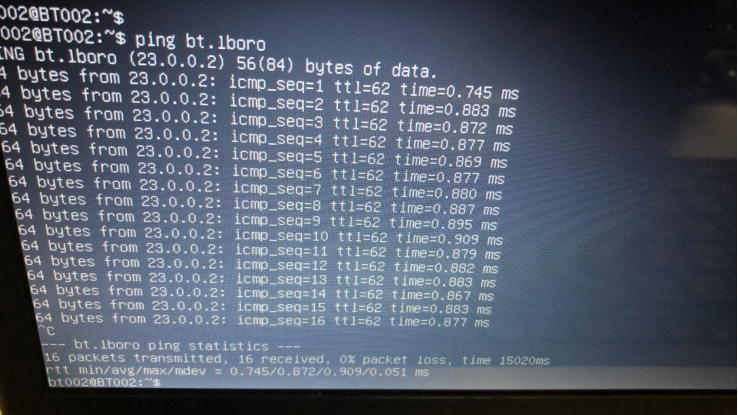
\includegraphics[width=\linewidth]{dns-ping-2}
	        \caption{Laptop 2 (BT002)}
	    \end{subfigure}
	    \\
	    \begin{subfigure}[b]{\linewidth}
	        \centering
	        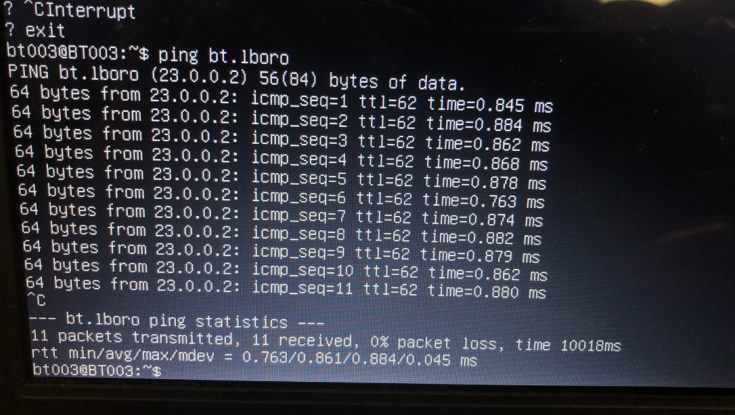
\includegraphics[width=\linewidth]{dns-ping-3}
	        \caption{Laptop 3 (BT003)}
	    \end{subfigure}
	\end{minipage}
    \caption{Connectivity to \texttt{bt.lboro} using \texttt{ping} on all $3$ Laptops.}
    \label{fig:dns-ping}
\end{figure*}








\subsection{Commentary}


\subsubsection{Problem: Querying IPv6 DNS Records}
Using \texttt{dig} directly does not return IPv6 addresses for domains. It turns out that \texttt{dig} queries \texttt{A} records by default. To query IPv6 DNS records, \texttt{dig AAAA domain-name} should be used.

\subsubsection{Problem: Reverse DNS Not Working}
Using \texttt{dig -x 23.0.0.2} does not return any answer initially.
It's later realized that the reverse DNS zone name has been wrongly set to \texttt{0.0.23.in-addr.arpa}.
To set up reverse DNS properly, the DNS zone should be \texttt{3.in-addr.arpa}. In addition, the first column for each DNS record inside file \texttt{db.23} should be the reverse host name (eg. \texttt{2.0.0} for IP address \texttt{23.0.0.2}). 



